\section{450 --- Delete Node in a BST}
Given a root node reference of a BST and a key $x$, delete the node with the given key in the BST. Return the root node reference (possibly updated) of the BST.

Basically, the deletion can be divided into two stages:

\begin{itemize}
\item Search for a node to remove.
\item If the node is found, delete the node.
\end{itemize}

\paragraph{Note:} 
\begin{itemize}
\item Time complexity should be O(height of tree).
\end{itemize}

\paragraph{Example:}
\begin{flushleft}
\textbf{Input}: 
\begin{figure}[H]
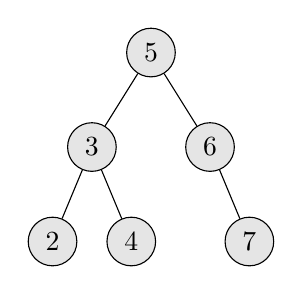
\begin{tikzpicture}
[every node/.style={draw, circle, fill=gray!20!, minimum size=5mm},
level 2/.style ={sibling distance=1cm}, 
level 3/.style={sibling distance=8mm},
level distance=1.2cm]
\node {5}
 child{ node(a){3} child { node {2} } child { node {4} }   } 
%
 child{ node(b){6} child[missing] {} child { node {7} } };
%;
\end{tikzpicture}
\end{figure}
$x = 3$

\textbf{Output}: 
One valid answer is shown in the following BST.

\begin{figure}[H]
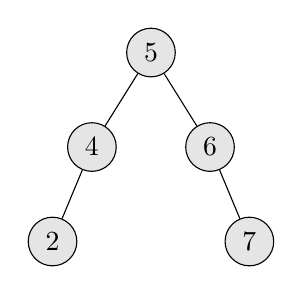
\begin{tikzpicture}
[every node/.style={draw, circle, fill=gray!20!, minimum size=5mm},
level 2/.style ={sibling distance=1cm}, 
level 3/.style={sibling distance=8mm},
level distance=1.2cm]
\node {5}
child { node {4} child {node{2}} child[missing]{} }
child { node {6} child[missing] {} child {node{7}} };
\end{tikzpicture}
\end{figure}

Another valid answer is
\begin{figure}[H]
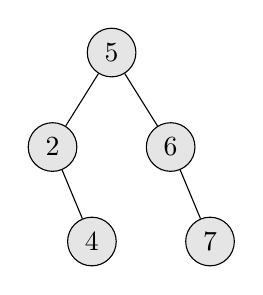
\begin{tikzpicture}
[every node/.style={draw, circle, fill=gray!20!, minimum size=5mm},
level 2/.style ={sibling distance=1cm}, 
level 3/.style={sibling distance=8mm},
level distance=1.2cm]
\node {5}
child { node {2} child[missing]{} child {node{4}} }
child { node {6} child[missing] {} child {node{7}} };
\end{tikzpicture}
\end{figure}
\end{flushleft}


\subsection{Recursion}
Here is list of facts which are better to know before the interview.
\begin{itemize}
\item Inorder traversal of BST is an array sorted in the ascending order.
\item To find a successor, go to the right once and then as many times to the left as you could.
\item  To find a predecessor, go to the left once and then as many times to the right as you could.
\end{itemize}

There are three possible situations here :

\begin{enumerate}
\item Node is a leaf, and one could delete it straightforward.
\item Node is not a leaf and has a right child. Then the node's value could be replaced by its successor which is somewhere lower in the right subtree. Then proceed down recursively to delete the successor.
\item Node is not a leaf, has no right child and has a left child. That means that its successor is somewhere upper in the tree but we don't want to go back. Let's use the predecessor here which is somewhere lower in the left subtree. The node's value could be replaced by its predecessor and then proceed down recursively to delete the predecessor.
\end{enumerate}

\setcounter{lstlisting}{0}
\begin{lstlisting}[style=customc, caption={Recursion}]
TreeNode* deleteNode( TreeNode* root, int key )
{
    if( !root )
    {
        return nullptr;
    }

    if( root->val < key )
    {
        //key is in the right child tree of root
        root->right = deleteNode( root->right, key );
    }
    else if( root->val > key )
    {
        //key is in the left child tree of root
        root->left = deleteNode( root->left, key );
    }
    else
    {
        //root is the node to be deleted
        if( !root->left && !root->right )
        {
            //root is leaf, just delete it
            delete root;
            root = nullptr;
        }
        else if( root->right )
        {
            //find the successor
            auto node = root->right;

            while( node->left )
            {
                node = node->left;
            }

            //replace root's val by the successor's value
            root->val = node->val;

            //delete sucessor from right child tree of root
            root->right = deleteNode( root->right, root->val );
        }
        else
        {
            //find the precessor
            auto node = root->left;
            while( node->right )
            {
                node = node->right;
            }

            //replace root's val by the successor's value
            root->val = node->val;

            //delete precessor from left child tree of root
            root->left = deleteNode( root->left, root->val );
        }

    }

    return root;

}
\end{lstlisting}